%%%%%%%%%%%%%%%%%%%%%%%%%%%%%%
% Laboratory report template %
% by Kamil Stokfiszewski     %
%%%%%%%%%%%%%%%%%%%%%%%%%%%%%%

\documentclass[12pt]{article}
\usepackage[T1]{fontenc}
\usepackage[cp1250]{inputenc}
\newcommand{\BibTeX}{{\sc Bib}\TeX} 
\usepackage{graphicx}
\usepackage{amsfonts}
\usepackage{textcomp}
\usepackage{listings}
\usepackage{xcolor}
\usepackage{courier}

\setlength{\textheight}{21cm}
\title{{\bf Assignment \textnumero$\:$1\linebreak 
The delta rule}\\\vspace{0.5cm}
\Large Intelligent Data Processing Laboratory}
\author{Maciej Socha, 239709 \textnumero$\:\!$ and Micha� Darowny, 239644 \textnumero}
\date{27.10.2021}

\begin{document}
\clearpage\maketitle
\thispagestyle{empty}
\newpage
\setcounter{page}{1}
\renewcommand{\ttdefault}{cmtt}

% general options of listings package - see listings package documentation
\definecolor{lst_backgrund_color}{RGB}{245,245,245}
\definecolor{lst_comment_color}{RGB}{0,140,255}
\definecolor{lst_numbers_color}{RGB}{120,120,120}
\definecolor{lst_strings_color}{RGB}{0,100,0}
\lstset
{
 language=Python,
 basicstyle=\footnotesize\ttfamily,
 keywordstyle=\color{blue}\bfseries,
 stringstyle=\color{lst_strings_color}\ttfamily,
 commentstyle=\color{lst_comment_color}\itshape,
 numberstyle=\color{lst_numbers_color}\ttfamily\bfseries,
 backgroundcolor=\color{lst_backgrund_color},
 numbers=left,
 stepnumber=1,
 firstnumber=1,
 numberfirstline=true,
 breaklines=true,
 showstringspaces=false,
 xleftmargin=0.75cm,
 xrightmargin=0.5cm,
 frame=trBL
}

\section{Main goal}

Our main goal was to implement and train with delta rule a linear neuron. To train neuron we used a simple and multiple training patterns.

\section{Theoretical background}

Every single linear neuron consist the following parts \cite{Instruction}:
\begin{enumerate}
	\item Vector of neurons inputs, $ x = [x_{1}, x_{2}, x_{3}, ... ,x_{n}] \in R^{N} $
	\item Vector of weights, $ w = [w_{1}, w_{2}, w_{3}, ... ,w_{n}] \in R^{N} $
	\item Output value, calculated: $ y = \sum w_{i} x_{i} $
\end{enumerate} 
In Figure \ref{Fig:neuron} there is a graphical representation of linear neuron.
\begin{figure}[h!]
 \centering
 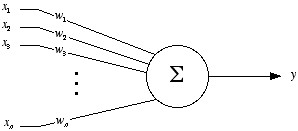
\includegraphics[width=9.3cm]{figures/linear-neuron.jpg}
 \vspace{-0.3cm}
 \caption{Linear neuron model}
 \label{Fig:neuron}
\end{figure}

The process of training can be carried out using single or multiple training patterns. In single our training set $ \Omega $ contains only one training pattern -- vector of inputs and desired output. With multiple training patterns $ \Omega $ contains many pairs of input vectors and desired outputs.

\section{Experiments and results}

We carry out experiments using single and multiple training patterns.

\subsection{Experiment \textnumero$\:$1}

\subsubsection{Description}

In this experiment we measured how changing of training step affects to results. We used a neuron with two inputs. Our training pattern was: $ \Omega = {[10, 10], 20} $. Number of epochs was 100.


\subsubsection{Results}

Table \ref{tab:ex1} presents calculated output for input vector $ x = [10, 10] $.

\begin{table}[h!]
\begin{tabular}{|c|c|c|c|c|c|}
\hline
Training step & Run 1      & Run 2      & Run 3      & Run 4      & Run 5      \\ \hline
0.1           & -3.85e+128 & -1.29e+129 & -1.13e+129 & -6.20e+128 & -3.07e+128 \\ \hline
0.01          & 13.57      & 12.63      & 8.93       & 4.95       & 9.33       \\ \hline
0.001         & 19.99      & 19.99      & 19.99      & 19.99      & 19.99      \\ \hline
\end{tabular}
\caption{Changing training step}
\label{tab:ex1}
\end{table}

As we can se, changing training step to lower number has positive impact to results. With $ \eta=0.001$ neuron calculates output properly.

\subsection{Experiment \textnumero$\:$2}

\subsubsection{Description}

In this experiment we measured how changing number of epochs affects to results. We used a neuron with two inputs. Our training pattern was: $ \Omega = \{[10, 10], 20\} $. Training step was set to 0.001.


\subsubsection{Results}

Table \ref{tab:ex2} presents calculated output for input vector $ x = [10, 10] $.

\begin{table}[h!]
\begin{tabular}{|c|c|c|c|c|c|}
\hline
Number of epochs & Run 1  & Run 2  & Run 3  & Run 4  & Run 5  \\ \hline
5      & 17.455 & 16.574 & 16.883 & 16.146 & 17.452 \\ \hline
25     & 19.954 & 19.942 & 19.943 & 19.928 & 19.949 \\ \hline
50     & 19.999 & 19.999 & 19.999 & 19.999 & 19.999 \\ \hline
\end{tabular}
\caption{Changing number of epochs}
\label{tab:ex2}
\end{table}

Higher number of epochs can help produce better results. In this example just 25 epochs give a quite good result.

\subsection{Experiment \textnumero$\:$3}


\subsubsection{Description}

We show how neuron works if we change number of inputs. We set training step to 0.001 and number of epochs to 50. In every run we used a training set:
\begin{enumerate}
	\item Run - $ \Omega = \{[5, 10], 15\}$
	\item Run - $ \Omega = \{[5, 10, 15], 30\}$
	\item Run - $ \Omega = \{[5, 10, 15, 20], 50\}$
	\item Run - $ \Omega = \{[5, 10, 15, 20, 25], 75\}$
\end{enumerate}

\subsubsection{Results}

\begin{table}[h!]
\begin{tabular}{|c|c|}
\hline
Run & Output             \\ \hline
1   & 14.995119228763564 \\ \hline
2   & 29.999999992876774 \\ \hline
3   & 50.0               \\ \hline
4   & 74.99999999999999  \\ \hline
\end{tabular}
\caption{Changing number of inputs}
\label{tab:ex3}
\end{table}

As table \ref{tab:ex3} shown, our implementation of neuron works with different numbers of input. The parameters we set work well with all of those training sets.

\subsection{Experiment \textnumero$\:$4}

\subsubsection{Description}

We set a number of epochs to 500 and training step to 0.0001. The neuron has 5 inputs. In this example we use a training set with three patterns $ \Omega = \{[[1, 2, 3, 4, 5], [10, 11, 12, 13, 14], [20, 21, 22, 23, 24]], [15, 60, 110]\}$

\subsubsection{Results}

\begin{table}[h!]
\centering
\begin{tabular}{|c|c|c|}
\hline
Input vector             & Calculated output  & Desired output \\ \hline
{[}1, 2, 3, 4, 5{]}      & 15.521469358995688 & 15             \\ \hline
{[}10, 11, 12, 13, 14{]} & 60.20899100373059  & 60             \\ \hline
{[}20, 21, 22, 23, 24{]} & 109.86179283121383 & 110            \\ \hline
{[}30, 31, 32, 33, 34{]} & 159.51459465869704 & 160            \\ \hline
{[}40, 41, 42, 43, 44{]} & 209.16739648618028 & 210            \\ \hline
{[}50, 51, 52, 53, 54{]} & 258.82019831366347 & 260            \\ \hline
{[}60, 61, 62, 63, 64{]} & 308.47300014114677 & 310            \\ \hline
\end{tabular}
\caption{3 training patterns}
\end{table}

\subsection{Experiment \textnumero$\:$5}

\subsubsection{Description}

We set a number of epochs to 500 and training step to 0.0001. The neuron has 5 inputs. In this example we use a training set with three patterns $ \Omega = \{[[1, 2, 3, 4, 5], [10, 11, 12, 13, 14], [20, 21, 22, 23, 24], [30, 31, 32, 33, 34], [40, 41, 42, 43, 44]], \newline [15, 60, 110, 160, 210]\}$

\subsubsection{Results}

\begin{table}[h!]
\centering
\begin{tabular}{|c|c|c|}
\hline
Input vector             & Calculated output  & Desired output \\ \hline
{[}1, 2, 3, 4, 5{]}      & 14.842336229272117 & 15             \\ \hline
{[}10, 11, 12, 13, 14{]} & 59.88041948415648  & 60             \\ \hline
{[}20, 21, 22, 23, 24{]} & 109.92273421180576 & 110            \\ \hline
{[}30, 31, 32, 33, 34{]} & 159.96504893945504 & 160            \\ \hline
{[}40, 41, 42, 43, 44{]} & 210.00736366710433 & 210            \\ \hline
{[}50, 51, 52, 53, 54{]} & 260.04967839475364 & 260            \\ \hline
{[}60, 61, 62, 63, 64{]} & 310.09199312240287 & 310            \\ \hline
\end{tabular}
\caption{5 training patterns}
\end{table}
\newpage
\subsection{Experiment \textnumero$\:$6}

\subsubsection{Description}

We set a number of epochs to 500 and training step to 0.0001. The neuron has 5 inputs. In this example we use a training set with three patterns $ \Omega = \{[[1, 2, 3, 4, 5], [10, 11, 12, 13, 14], [20, 21, 22, 23, 24], [30, 31, 32, 33, 34], [40, 41, 42, 43, 44], \newline [50, 51, 52, 53, 54], [60, 61, 62, 63, 64]], [15, 60, 110, 160, 210, 260, 310]\}$

\subsubsection{Results}

\begin{table}[h!]
\centering
\begin{tabular}{|c|c|c|}
\hline
Input vector             & Calculated output  & Desired output \\ \hline
{[}1, 2, 3, 4, 5{]}      & 15.234540131857925 & 15             \\ \hline
{[}10, 11, 12, 13, 14{]} & 60.201467346657466 & 60             \\ \hline
{[}20, 21, 22, 23, 24{]} & 110.16471980754585 & 110            \\ \hline
{[}30, 31, 32, 33, 34{]} & 160.12797226843423 & 160            \\ \hline
{[}40, 41, 42, 43, 44{]} & 210.09122472932262 & 210            \\ \hline
{[}50, 51, 52, 53, 54{]} & 260.05447719021095 & 260            \\ \hline
{[}60, 61, 62, 63, 64{]} & 310.01772965109933 & 310            \\ \hline
\end{tabular}
\caption{7 training patterns}
\end{table}

\section{Summary and conclusions}

\begin{itemize}
	\item Higher number of epochs has positive impact on results
	\item Lower training step help to give a more accurate results
	\item More training patterns give us a better results, but it would be greate to check it for more different patterns
\end{itemize}

\bibliographystyle{plain}
\bibliography{bibliography}

\end{document}
